%%%%%%%%%%%%%%%%%%%%%%%%%%%%%%%%%%%%%%%%%%%%%%%%%%%%%%%%%%%%%%%%%%%%%%%%%%%%%%%%
%2345678901234567890123456789012345678901234567890123456789012345678901234567890
%        1         2         3         4         5         6         7         8

\documentclass[letterpaper, 10 pt, conference]{ieeeconf}  % Comment this line out
                                                          % if you need a4paper
%\documentclass[a4paper, 10pt, conference]{ieeeconf}      % Use this line for a4
                                                          % paper

\IEEEoverridecommandlockouts                              % This command is only
                                                          % needed if you want to
                                                          % use the \thanks command
\overrideIEEEmargins
% See the \addtolength command later in the file to balance the column lengths
% on the last page of the document



% The following packages can be found on http:\\www.ctan.org
%\usepackage{graphics} % for pdf, bitmapped graphics files
%\usepackage{epsfig} % for postscript graphics files
%\usepackage{mathptmx} % assumes new font selection scheme installed
%\usepackage{times} % assumes new font selection scheme installed
%\usepackage{amsmath} % assumes amsmath package installed
%\usepackage{amssymb}  % assumes amsmath package installed
\usepackage{amsmath,amsthm,amssymb, graphicx, multicol, array}

\title{\LARGE \bf
TopCoder Ideation Challenge: Purple Kernel Monsters
}

\author{Zhiwei Zhang, Kathir Gounder, Yongming Ge % 
}

\begin{document}

\maketitle
\thispagestyle{empty}
\pagestyle{empty}

\section{Introduction}

This is first and foremost an image classification problem, so from a high level we will treat it as such. But there is also a significant carpological component to the task, so to provide the challenge creators with novel ideas and possible solution avenues rather than a bombardment of machine learning methods (that they are probably aware of) we focused the bulk of our effort in indepth literature review.  

We surveyed procedures and results from a few significant papers in the agricultural data analysis space, especially the practice of predicting seed viability (i.e potential for germination) \cite{DBLP:journals/cea/PrzybyloJ19},\cite{Jablonski2016ColourBasedBD},\cite{liao2018hyperspectral}. Even though we do not know the exact botany behind the purple kernel challenge, after talking to some agriculture professors here at UC Berkeley and Cal Poly SLO and taking into account that the images were only one day apart, we theorized that the purple kernels were seeds actually germinating. This might be completely wrong however, maybe the purple color is a fungal infection and so on but we still decided that seed viability would be a good jumping off point as the data analysis techniques are transferable. The most important element to this problem based on our research is color information. Within color information are contained other implicit features such as size and shape. So the way in which this information is handled becomes the most dividing factor among model choice. 

Following our studies and our few experiments we recommend to the challenge creators two potential classification procedures: a simple Naive Bayes classifier or a deep transfer learning model (CNN-F-IMAGENET). A baseline accuracy threshold we used when considering models was 75\%. The accuracy score we were able to achieve from educated human guessing using the hints given by the challenge creator was 68\% but we added 5\% to the threshold to emulate that classification procedure of a somewhat seed-expert. The oakcorn classifaction experts from the papers we read were achieving accuracy scores of 80-84\%. When looking at possible The choice of which classifier surprisingly does not depend on desired accuracy as both the surveyed deep learning models and traditional ML image analysis methods were hovering around the certain. But rather the choice depends on certain questions: Are image preprocessing methods available (these can get complicated), what are the specifications of the system in which the classifier will be run, are the users interested in extracting/learning about features or just classifying seeds etc. More specifically how much information are we willing to collect and give to the model, deep learning models are pretty much hands off when compared to traditional image analysis methods but the trade off is that we do not learn much about said images. We will provide the necessary information and ideas for the user to make an informed decision regarding model choice. We have also provided code for the challenege creators to segment their petri dish images into individual seeds for convenient model training and prediction greatly increasing the speed of the entire process. 

\section{Traditional Image Analysis (Naive Bayes)}

Procedures utilizing shape, length, diameter and
density to predict seed viability have been proven to be ineffecient. \cite{Jablonski2016ColourBasedBD},\cite{DBLP:journals/cea/PrzybyloJ19} show that changes in color information such as the average components of the RGB space, and perception-based based hue-saturation-value
colour space.

Due to the importance of color information, we have to make sure to remove the effects of background lighting and varying information. Traditional Image Analysis works well only if unnecessary information i.e noise is removed as much as possible. The quality of the colour information represented by hue is dependent on several factors, mainly on ambient illumination and the properties of the camera image sensor. The camera setup here becomes extremely crucial and could be the limiting component. But we also believe that a good preprocessing pipeline can overcome a bad camera set up i.e the one in the purple kernel challenge. 

{\centering 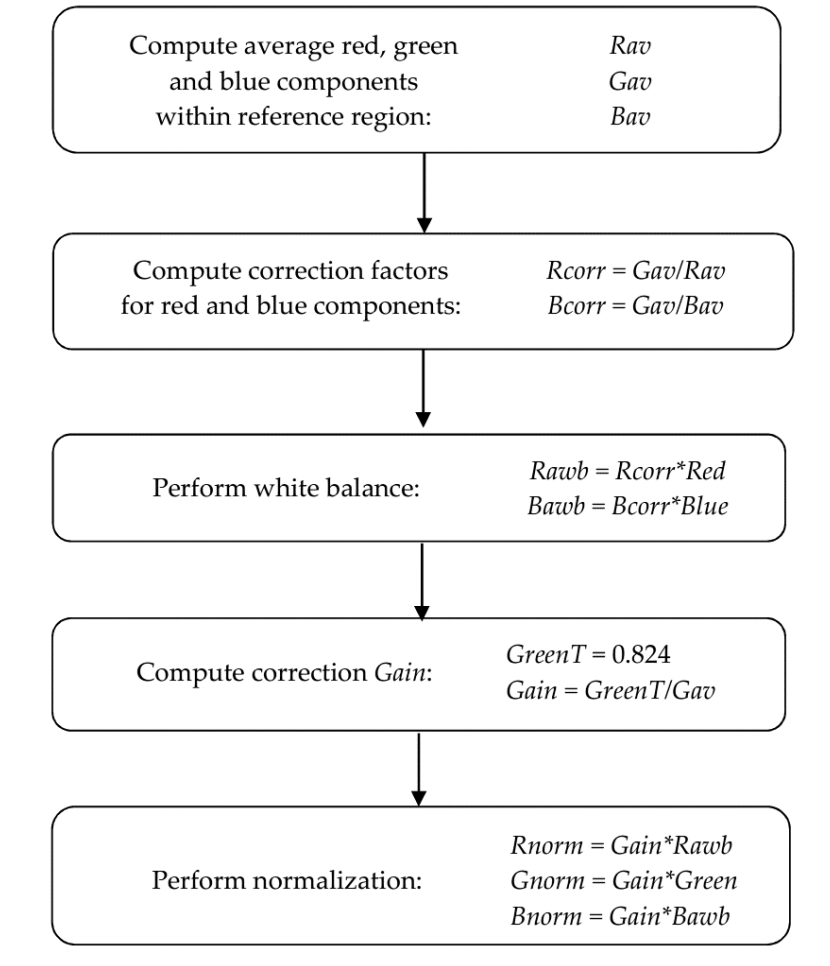
\includegraphics[scale = 0.4]{preprocessing.png} \par}
\cite{Jablonski2016ColourBasedBD} recommends this specific pipeline 
``(a) white balance; (b) normalization; (c) colour space transformation;
(d) segmentation (determining rectangular and circular ROIs); (e) computation of scalar features; and
(f) prediction of viability and analysis of results combined with experimental germination data." Out of these we found that white balancing and normalisation are absolutely crucial (even in the deep learning formulation) to balance illumination and remove the effects of lighting changes. The authors of the paper used image segmentation to target specific blots or blemishes on their oakcorn seeds. We instead target the lighter areas of the kernels. From elementary analysis these areas seem to carry a lot of information regarding the future status of the kernel. Normalization led to an almost ten percent increase in accuracy. 

To work with individual kernels and create a viable dataset we have provided the challenge creators with image segmentation code

\subsubsection{Cropping Kernels}
To single out the image of each kernel, we use OpenCV to crop them out. However, it's difficult to apply a single algorithm to every image as they have different illumination details and we have to manually tell the program to target what pixel values.
In addition, since we crop out kernels of the first day and the second day, we have make sure that we crop them in the same order. We resolve this by sorting the kernels first by their $x$-coordinate then their $y$-coordinate.
\subsubsection{Labeling}
We manually labelled the images, which honeslty was not too bad. But a faster way to do it would be a simple purple hue detection algorithm (i.e specific color range). If any purple is detected for example we could label it as such. Imageset labelling is its own field of study, we could potentially even train another neural network to do the labelling. 

After this is all done, it is simple to formulate a naive bayes classifier with the data. A library that we used for experiments is sklearn, it makes for rapid prototyping and very good perfomance as well. The research shows that some image processing methods can greatly improve accuracy: 
\begin{enumerate}
    \item White Balance: reduce hue information
    \item Brightness Normalization: improves overall accuracy 
\end{enumerate}
Jablonski et.al in their research show that Naive Bayes training algorithm has a similar accuracy as professionals when determining germination of \textit{Quercus robur} acorns by observing their cross section image\cite{Jablonski2016ColourBasedBD}. Similarly, we should also consider using Naive Bayes training algorithm.

\section{Deep Learning Techniques}

Using a deep learning model such as a convolutional neural network provides certain conveniences when compared to previous approaches, is that beside basic image dataset preparation, it does not require any substantial preprocessing. It takes in the input and simply puts out the prediction: purple kernel or not. 

Based on the popular research we think an ordinary CNN architecture is sufficient to achieve expert results and extract basic features such as global intensity or colour components on its own. \cite{DBLP:journals/cea/PrzybyloJ19} shows that spatial structure of an image is important for classification which further supports the choice of a CNN as CNNs are spatially invariant when it comes to detecting features. 


Before Deep Neural Network training, an image normalisation of the data sets is performed. Typical image normalisation is to zero-centre the data and then normalise them to a z-score. We suggest using additional entropy filtering as well. 

The only issue with the deep learning formulation is that we need a large dataset as neural networks optimize somewhat slowly. We and the a lot of the authors in literature have only a few hundred images. To tackle this issue of sparse data, we recommend using some basic data augmentation techniques such as mirroring (color information is kept intact) and transfer learning. 

The idea of transfer learning is to apply the relevant knowledge from previous learning experiences when encountering a new task. Large CNNs that have been trained on massive data sets to recognize thousands of different categories are master generalized feature extractors (or atleast their lower convolutional layers are). So we can take these pretrained layers and attach to them regular untrained fully connected layers designed for our specific classification task. In other words, the pretrained layers extract features and the newly added FC layers are trained to classify images based on these extracted features. It is a simple and a somewhat ingenious idea. 

 The highest accuracy was obtained for training images in RGB colour space with white balance, brightness equalisation and scaling (AWB\_RGB).

In conclusion, we show that deep network accuracy (85\%) is comparable or slightly higher than the manual predictions of the human experts. Although the accuracy of recognition by means of Deep CNN was not considerably better than other computer based or visual methods it has a lot bonuses. The advantage of using a CNN for seed classification is that beside image segmentation and normalization, it does not Also, it proves that computer methods, including machine learning, are as accurate as humans in vision-based assessment of acorn viability and faster than employees. The training procedure is time-consuming but the recognition task takes 68 ms on average.

\nocite{*}
\bibliographystyle{IEEEannot}
\bibliography{annot}

\end{document}
